% Meta-Informationen -------------------------------------------------------
%    Informationen über das Dokument, wie z.B. Titel, Autor, Matrikelnr. etc
%    werden in der Datei _Meta.tex definiert und können danach global
%    verwendet werden.
% --------------------------------------------------------------------------
% Informationen ------------------------------------------------------------
%   Definition von globalen Parametern, die im gesamten Dokument verwendet
%   werden können (z.B auf dem Deckblatt etc.).
% --------------------------------------------------------------------------
\newcommand{\titel}{Use of Imitation Learning in an Obstacle Course Scenario}
\newcommand{\art}{Bachelor Thesis}
\newcommand{\ort}{Leipzig}
\newcommand{\hochschule}{Leipzig University}
\newcommand{\fachgebiet}{Database Department}
\newcommand{\fakultaet}{Faculty of Mathematics and Computer Science}
\newcommand{\institut}{Institute of Computer Science}
\newcommand{\autor}{Andrian Yarotskyi}
\newcommand{\matrikelnr}{3740921}
\newcommand{\erstbetreuer}{Dr. Thomas Burghardt}
\newcommand{\jahr}{2025}
\newcommand{\invnr}{1337}
\newcommand{\eingereicht}{xx.xx.xxxx}

% Eigene Befehle
\newcommand{\todo}[1]{\textbf{\textsc{\textcolor{red}{(TODO: #1)}}}}

% Autorennamen in small caps
\newcommand{\AutorZ}[1]{\textsc{#1}}
\newcommand{\Autor}[1]{\AutorZ{\citeauthor{#1}}}

% Befehle zur semantischen Auszeichnung von Text
\newcommand{\NeuerBegriff}[1]{\textbf{#1}}
\newcommand{\Fachbegriff}[1]{\textit{#1}}
\newcommand{\Prozess}[1]{\textit{#1}}
\newcommand{\Webservice}[1]{\textit{#1}}
\newcommand{\Eingabe}[1]{\texttt{#1}}
\newcommand{\Code}[1]{\texttt{#1}}
\newcommand{\Datei}[1]{\texttt{#1}}
\newcommand{\Datentyp}[1]{\textsf{#1}}
\newcommand{\XMLElement}[1]{\textsf{#1}}

% Abkürzungen
\newcommand{\vgl}{Vgl.\ }
\newcommand{\ua}{\mbox{u.\,a.\ }}
\newcommand{\zB}{\mbox{z.\,B.\ }}
\newcommand{\bs}{$\backslash$}

% Einfache Anführungszeichen in texttt
\newcommand{\sq}{\textquotesingle}


% Dokumentenkopf -----------------------------------------------------------
%   Diese Vorlage basiert auf "scrreprt" aus dem koma-script.
%    Die Option draft sollte beim fertigen Dokument ausgeschaltet werden.
% --------------------------------------------------------------------------
\documentclass[
  11pt,          % Schriftgröße
  DIV=10,
  english,        % für Umlaute, Silbentrennung etc.
  a4paper,        % Papierformat
  oneside,        % einseitiges Dokument
  titlepage,        % es wird eine Titelseite verwendet
  parskip=half,      % Abstand zwischen Absätzen (halbe Zeile)
  headings=normal, % Größe der Überschriften verkleinern
  numbers=withendperiod, % Fügt in den Überschriften nach den Zahlen einen Punkt ein
  listof=totoc,        % Verzeichnisse im Contentsverzeichnis aufführen
  bibliography=totoc,        % Literaturverzeichnis im Contentsverzeichnis aufführen
  index=totoc,        % Index im Contentsverzeichnis aufführen
  captions=tableheading,    % Beschriftung von Tabellen oberhalb ausgeben
  final          % Status des Dokuments (final/draft)
]{scrreprt}

\renewcommand*\chapterheadstartvskip{\vspace*{-1.0cm}}

% Bentigte Packages -------------------------------------------------------
%    Weitere Packages, die benötigt werden, sind in die Datei Packages.tex
%    "ausgelagert", um die Vorlage möglichst übersichtlich zu halten.
% --------------------------------------------------------------------------
% Anpassung des Seitenlayouts ----------------------------------------------
%   siehe Seitenstil.tex
% --------------------------------------------------------------------------
\usepackage[
  automark,      % Kapitelangaben in Kopfzeile automatisch erstellen
  headsepline,  % Trennlinie unter Kopfzeile
  ilines        % Trennlinie linksbündig ausrichten
]{scrlayer-scrpage}
\usepackage{scrhack} % Disable some warnings

\usepackage{pseudocode}
\usepackage{nicefrac}

% Für eine schöne Anordnung von Bildern
\usepackage{subfigure}

\usepackage{dsfont}
%\usepackage{color}
%
%% Define user colors using the RGB model
%\definecolor{yellow}{rgb}{0.0,1.0,0.0}
%\definecolor{rot}{rgb}{1.0,0.0,0.0}

% Anpassung an Landessprache -----------------------------------------------
%   Verwendet globale Option german siehe \documentclass
% --------------------------------------------------------------------------
\usepackage[english]{babel}

% Umlaute ------------------------------------------------------------------
%     Umlaute/Sonderzeichen wie äöüß direkt im Quelltext verwenden (CodePage).
%    Erlaubt automatische Trennung von Worten mit Umlauten.
% --------------------------------------------------------------------------
\usepackage[utf8]{inputenc}
\usepackage[T1]{fontenc}
%\usepackage{ae} % "schöneres" ä
\usepackage{textcomp} % Euro-Zeichen etc.
\usepackage{lmodern} % schööön

% Grafiken -----------------------------------------------------------------
%     Einbinden von Grafiken [draft oder final]
%     Option [draft] bindet Bilder nicht ein - auch globale Option
% --------------------------------------------------------------------------
\usepackage[dvips,final]{graphicx}
\usepackage{wrapfig}
\graphicspath{{Images/}} % Dort liegen die Bilder des Dokuments

% Befehle aus AMSTeX für mathematische Symbole z.B. \boldsymbol \mathbb ----
\usepackage{amsmath,amsfonts,amsthm}

% Für Index-Ausgabe; \printindex -------------------------------------------
\usepackage{makeidx}

% Einfache Definition der Zeilenabstände und Seitenränder etc. -------------
\usepackage{setspace}
\usepackage{geometry}

% für gedrehte Tabellen
\usepackage{rotating}

% Symbolverzeichnis --------------------------------------------------------
%   Symbolverzeichnisse bequem erstellen, beruht auf MakeIndex.
%     makeindex.exe %Name%.nlo -s nomencl.ist -o %Name%.nls
%   erzeugt dann das Verzeichnis. Dieser Befehl kann z.B. im TeXnicCenter
%    als Postprozessor eingetragen werden, damit er nicht ständig manuell
%    ausgeführt werden muss.
%    Die Definitionen sind ausgegliedert in die Datei Abkuerzungen.tex.
% --------------------------------------------------------------------------
\usepackage[intoc]{nomencl}
\let\abbrev\nomenclature
\renewcommand{\nomname}{Abkürzungsverzeichnis}
\setlength{\nomlabelwidth}{.25\hsize}
\renewcommand{\nomlabel}[1]{#1 \dotfill}
\setlength{\nomitemsep}{-\parsep}

% Zum Umfließen von Bildern -------------------------------------------------
\usepackage{floatflt}

% Zum Einbinden von Programmcode --------------------------------------------
\usepackage{listings}
\usepackage{xcolor}
\definecolor{hellgelb}{rgb}{1,1,0.9}
\definecolor{colKeys}{rgb}{0,0,1}
\definecolor{colIdentifier}{rgb}{0,0,0}
\definecolor{colComments}{rgb}{1,0,0}
\definecolor{colString}{rgb}{0,0.5,0}
\lstset{%
  float=hbp,%
  basicstyle=\texttt\small, %
  identifierstyle=\color{colIdentifier}, %
  keywordstyle=\color{colKeys}, %
  stringstyle=\color{colString}, %
  commentstyle=\color{colComments}, %
  columns=flexible, %
  tabsize=2, %
  frame=single, %
  extendedchars=true, %
  showspaces=false, %
  showstringspaces=false, %
  numbers=left, %
  numberstyle=\tiny, %
  breaklines=true, %
  backgroundcolor=\color{hellgelb}, %
  breakautoindent=true, %
  %    captionpos=b%
}

% Lange URLs umbrechen etc. -------------------------------------------------
\usepackage{url}

%% Wichtig für korrekte Zitierweise ------------------------------------------

\usepackage[autocite=inline, sorting=none]{biblatex}
\bibliography{sources} % Name der .bib-Datei

\usepackage{csquotes} % Empfohlen, um Zitierten Text richtig darzustellen

% ermöglicht Zeilenumbrüche in Captions
\usepackage{caption}

% PDF-Optionen --------------------------------------------------------------
\usepackage[
  bookmarks,
  bookmarksopen=true,
  pdftitle={\titel},
  pdfauthor={\autor},
  pdfcreator={\autor},
  pdfsubject={\titel},
  pdfkeywords={\titel},
  colorlinks=true,
  %linkcolor=red, % einfache interne Verknüpfungen
  %anchorcolor=black,% Ankertext
  %citecolor=blue, % Verweise auf Literaturverzeichniseinträge im Text
  %filecolor=magenta, % Verknüpfungen, die lokale Dateien öffnen
  %menucolor=red, % Acrobat-Menüpunkte
  %urlcolor=cyan,
  % für die Druckversion können die Farben ausgeschaltet werden:
  linkcolor=black, % einfache interne Verknüpfungen
  anchorcolor=black,% Ankertext
  citecolor=black, % Verweise auf Literaturverzeichniseinträge im Text5
  filecolor=black, % Verknüpfungen, die lokale Dateien öffnen
  menucolor=black, % Acrobat-Menüpunkte
  urlcolor=black,
  %backref,
  %pagebackref,
  plainpages=false,% zur korrekten Erstellung der Bookmarks
  pdfpagelabels,% zur korrekten Erstellung der Bookmarks
  hypertexnames=false,% zur korrekten Erstellung der Bookmarks
  linktocpage % Seitenzahlen anstatt Text im Inhaltsverzeichnis verlinken
]{hyperref}

% Zum fortlaufenden Durchnummerieren der Fußnoten ---------------------------
\usepackage{chngcntr}

% für lange Tabellen
\usepackage{longtable}
\usepackage{array}
\usepackage{ragged2e}
\usepackage{lscape}

\usepackage{supertabular}

% Spaltendefinition rechtsbündig mit definierter Breite ---------------------
\newcolumntype{w}[1]{>{\raggedleft\hspace{0pt}}p{#1}}

% Formatierung von Listen ändern
\usepackage{paralist}
% Standardeinstellungen:
% \setdefaultleftmargin{2.5em}{2.2em}{1.87em}{1.7em}{1em}{1em}

\usepackage{tablefootnote}
% für Ausblenden der Seitenzahl
\usepackage{lipsum}
\usepackage{algorithm}
\usepackage{algpseudocodex}
\usepackage{tabu}

% Erstellung eines Index und Abkürzungsverzeichnisses aktivieren -----------
\makeindex
% makeindex Bachelorarbeit.nlo -s nomencl.ist -o Bachelorarbeit.nls
\makenomenclature

% Kopf- und Fußzeilen, Seitenränder etc. -----------------------------------
% Zeilenabstand ------------------------------------------------------------
\onehalfspacing
% \setstretch{1,5}

% Seitenränder -------------------------------------------------------------
\geometry{paper=a4paper,left=25mm,right=20mm,top=20mm, bottom=25mm}
% Notfall maße :)
%\geometry{paper=a4paper,left=35mm,right=25mm,top=25mm, bottom=25mm}

% Kopf- und Fußzeilen ------------------------------------------------------
\pagestyle{scrheadings}

% Kopf- und Fußzeile auch auf Kapitelanfangsseiten -------------------------
\renewcommand*{\chapterpagestyle}{scrheadings}

% Schriftform der Kopfzeile ------------------------------------------------
\renewcommand{\headfont}{\normalfont}

% Kopfzeile ----------------------------------------------------------------
\ihead{\textit{\headmark}}
\chead{}
%\ohead{\includegraphics[scale=1]{Bilder/logoKlein.JPG}}
\ohead{}
\setlength{\headheight}{8mm} % Höhe der Kopfzeile
\setheadwidth[0pt]{textwithmarginpar} % Kopfzeile über den Text hinaus verbreitern

% Fußzeile -----------------------------------------------------------------
% \ifoot{\copyright\ \autor \\ \invnr}
% \ifoot{\copyright\ \autor \\ \matrikelnr}
\ifoot{\autor \\ \matrikelnr}
\cfoot{}
\ofoot{\pagemark}
\setlength{\footskip}{12mm}
\setfootwidth[0pt]{text}

% Überschriften ------------------------------------------------------------
\renewcommand*\chapterheadstartvskip{\vspace*{-0.5cm}} % Platz vor einer Überschrift eines neuen Kapitels

% erzeugt ein wenig mehr Platz hinter einem Punkt --------------------------
\frenchspacing

% Schusterjungen und Hurenkinder vermeiden
\clubpenalty = 10000
\widowpenalty = 10000
\displaywidowpenalty = 10000

% Quellcode-Ausgabe formatieren --------------------------------------------
%\lstset{numbers=left, numberstyle=\tiny, numbersep=5pt, breaklines=true}
%\lstset{emph={square}, emphstyle=\color{red}, emph={[2]root,base}, emphstyle={[2]\color{blue}}}

\definecolor{gray}{rgb}{0.9,0.9,0.9}

\lstset{%
  basicstyle=\small\ttfamily,language={[LaTeX]TeX},
  numbersep=5mm,
  numbers=left,
  numberstyle=\tiny,
  breaklines=true,
  framexleftmargin=8mm,
  xleftmargin=8mm,
  backgroundcolor=\color{gray},
  captionpos=b
}%

% Fußnoten fortlaufend durchnummerieren ------------------------------------
\counterwithout{footnote}{chapter}

% Definitionen

\newtheorem{definition}{Definition}


\begin{document}
% Eigene Definitionen für Silbentrennung
\hyphenation{Trenn-bar-es}

% Das eigentliche Dokument -------------------------------------------------
%    Der eigentliche Content des Dokuments beginnt hier. Die einzelnen Seiten
%    und Kapitel werden in eigene Dateien ausgelagert und hier nur inkludiert.
% --------------------------------------------------------------------------
% auch subsubsection nummerieren
\setcounter{secnumdepth}{3}
\setcounter{tocdepth}{3}

% keine Kopf-/Fußzeilen bei Deckblatt und Abstract
\ofoot{}
% Deckblatt
\thispagestyle{plain}
\begin{titlepage}

  \begin{center}
    
\includegraphics[height=7cm]{Bilder/Uni-L.png}\\[2.5ex]

    \hochschule\\
    \institut\\
    \fakultaet\\
    \fachgebiet\\[6ex]

    \textbf{\large\titel}\\[1.5ex]
    \art\\[6ex]

    \normalsize
    Submitted by:\\
    \autor\\[1.5ex]
    Matriculation number:\\
    \matrikelnr\\[1.5ex]
    Supervisor:\\
    \erstbetreuer\\
    \zweitbetreuer\\[1.0ex]
  \end{center}

  %\begin{tabbing}
  %\hspace{3.5cm}\= \kill
  %   vorgelegt von: \> \autor\\[1.2ex]
  %   Matrikelnummer: \> \matrikelnr\\[1.2ex]
  %    \> \\
  %   Betreuer: \> \erstbetreuer\\[1.2ex]
  %    \> \zweitbetreuer
  %\end{tabbing}

  \begin{center}
    \copyright\ \jahr\\[1.0ex]
  \end{center}

  \singlespacing
  \small
  \noindent This work including its parts is \textbf{protected by copyright}. Any use outside the narrow limits of copyright law without the consent of the author is prohibited and punishable. This applies in particular to duplications, translations, microfilming and storage and processing in electronic systems.

\end{titlepage}


\section*{Zusammenfassung}
\label{sec:Zusammenfassung}

Zusammenfassung meiner Arbeit hier....
\ofoot{\pagemark}

% Seitennummerierung -------------------------------------------------------
%    Vor dem Hauptteil werden die Seiten in großen römischen Ziffern
%    nummeriert...
% --------------------------------------------------------------------------
\pagenumbering{Roman}

\tableofcontents      % Contentsverzeichnis

% Abkürzungsverzeichnis ----------------------------------------------------
%\input{Content/Glossar}
%\printnomenclature
%\label{sec:Glossar}

\listoffigures          % Abbildungsverzeichnis
\listoftables          % List of tables

%\renewcommand{\lstlistlistingname}{Verzeichnis der Listings}
%\lstlistoflistings

% ...danach in normalen arabischen Ziffern ---------------------------------
\clearpage
\pagenumbering{arabic}

% Content -------------------------------------------------------------------
%    Hier können jetzt die einzelnen Kapitel inkludiert werden. Sie müssen
%    in den entsprechenden .TEX-Dateien vorliegen. Die Dateinamen können
%     natürlich angepasst werden.
% --------------------------------------------------------------------------
\chapter{Introduction}
\label{cha:Introduction}

\section{Motivation}

\section{Goals of the thesis}

\section{Structure of the thesis}

To assess the generalization abilities of the model the 2 levels of difficulties for the agent are introduced:
\begin{enumerate}
  \item \textbf{First level of difficulty:} In this setting the vehicle always starts from a certain position and the obstacles are also fixed at predetermined positions. This level of difficulty is used to test the basic skills of the model. As the environment remains constant, the robot can learn stable behavior through repeated training.
  \item \textbf{Second level of difficulty:} In this setting the positions of both the robot and the obstacles will vary in a random fashion. On this level the generalization abilities of the model will be tested. Since each drive is performed differently and not in a way in which the model was trained, this difficulty level challenges the model's ability to spot and analyze more general features and not just to rely on memorization.
\end{enumerate}

The research is aimed to put clearness in the following questions: (1) Can the model be trained using Behavioral Cloning \autocite{8855753} to demonstrate human performance or even surpass it in the first difficulty? (2) Can the model be sufficiently generalized using behavioral cloning to demonstrate human performance or even surpass it in the second difficulty? (3) Can the Inverse Reinforcement Learning (IRL) \autocite{ng2000algorithms} \autocite{neu2012apprenticeshiplearningusinginverse} \autocites{lee2021approximateinversereinforcementlearning} approach eliminate the expected weaknesses of the Behavioral Cloning approach in mastering the course on both difficulty levels and contribute to successfully mastering the course? \\
The last question will be answered with a help of literature, since there is no possibility to implement IRL algorithms in current settings.

\chapter{Background}
\label{cha:Background}

\section{Deep learning}

\begin{definition}
  An \textit{Artificial Neural Network (ANN)} \autocite{oshea2015introductionconvolutionalneuralnetworks} \autocite{sharma2017activation} is a computational model inspired by the structure and function of biological neural networks. It consists of interconnected artificial neurons (or nodes), which collectively process input data and learn patterns through training.

  In the case of Feedforward Neural Networks (FNNs), neurons are organized into layers, with each neuron in one layer connected to every neuron in the subsequent layer via directed connections. These connections are associated with trainable parameters called weights. Other neural architectures, such as Restricted Boltzmann Machines (RBMs) and Recurrent Neural Networks (RNNs), use different strategies for grouping and connecting neurons to capture specific data structures or temporal dependencies.

  Each neuron in the network also possesses a bias term—another learnable parameter—used to adjust the activation threshold. The output of a neuron is computed as a function of the weighted sum of its inputs and its bias, passed through a non-linear activation function. During training, both weights and biases are updated to minimize the network’s prediction error and improve its performance.
\end{definition}

\begin{definition}
  An \textit{Activation Function} \autocite{sharma2017activation} is a mathematical function used in artificial neural networks to determine the output of a neuron based on its input, associated weights, and bias. Given a neuron with inputs \(x\), weights \(w\), and bias \(b\), the neuron computes a linear combination \(z = w^\top x + b\). The activation function is then applied to this linear output, producing the final output of the neuron. Activation functions introduce non-linearity into the network, enabling it to learn complex patterns and approximate arbitrary functions. Common activation functions include the Sigmoid, Hyperbolic Tangent (Tanh), and Rectified Linear Unit (ReLU).
\end{definition}

An activation function is typically expected to exhibit two key mathematical properties:
\begin{enumerate}
  \item \textbf{Nonlinearity} \autocite{augustine2024surveyuniversalapproximationtheorems}: To satisfy the conditions of the Universal Approximation Theorem and enable the network to model complex, non-linear relationships, activation functions must introduce nonlinearity into the system. Using a nonlinear activation function in hidden layers is essential for learning intricate patterns in the data, but linear functions are also sometimes used, e.g. in the output layer of neural networks.
  \item \textbf{Differentiability} \autocite{sharma2017activation}: The activation function should ideally be differentiable across its entire domain to allow the computation of gradients during backpropagation. This is necessary for calculating loss gradients with respect to the network’s weights, enabling optimization techniques like Gradient Descent. However, it is not strictly necessary for the function to be continuously differentiable. For instance, the Rectified Linear Unit (ReLU) is not differentiable at zero, yet it is widely used—particularly in combination with convolutional layers—due to its empirical effectiveness and computational efficiency \autocite{alzubaidi2021review}.
\end{enumerate}

\begin{definition}
  \textit{Deep supervised learning} \autocite{alzubaidi2021review} \autocite{cun2015deeplearning} \autocite{oshea2015introductionconvolutionalneuralnetworks} is a machine learning approach that relies on labeled data to train deep neural networks. Let \(D_t\), denote the training dataset, where each example \((x_t, y_t) \in D_t\) consists of an input datapoint \(x_t\) and its corresponding output label \(y_t\). A function \(f\), typically represented by an artificial neural network (ANN), is learned to map inputs to outputs. The discrepancy between the predicted output \(f(x_t)\) and the true output \(y_t\) is quantified using a loss function \(\gamma\), yielding a loss value \(\gamma(y_t, f(x_t))\). Optimization techniques such as Gradient Descent are then used to iteratively update the network’s parameters in order to minimize the loss, thereby improving the model’s accuracy in approximating the target function.
\end{definition}

\section{Convolutional Neural Networks}

Convolutional Neural Networks (CNNs) are among the most widely used and powerful tools in the field of Computer Vision. They excel at tasks such as image classification, dimensionality reduction, and other operations involving high-dimensional data. One of their key advantages is the ability to efficiently extract meaningful features from images without the need to store vast numbers of parameters, making them highly effective for analyzing complex, multidimensional data. While CNNs are primarily designed for processing two-dimensional inputs, they can also be adapted for one-dimensional \autocite{8126078} or three-dimensional \autocite{9786658} data, enabling their use in applications like sequence prediction and volumetric data classification.

\begin{definition}
  A \textit{kernel} \autocite{alzubaidi2021review}, also known as filter, is a small matrix of learnable weights $K \in \mathbb{R}^{m \times n}$ (or a higher-dimensional tensor, depending on the input) used in the convolutional and pooling layers of a Convolutional Neural Network (CNN). In convolutional layers it performs the convolution operation by sliding across the input $X$, computing a dot product at each position:
  \[(X * K)(i, j) = \sum_{u=0}^{m-1} \sum_{v=0}^{n-1} X(i+u, j+v) \cdot K(u, v) \]
  This operation produces a feature map that highlights spatial patterns such as edges or textures. The kernel weights are optimized during training.
\end{definition}

\begin{definition}
  A \textit{convolutional operation} \autocite{alzubaidi2021review} is a process in which a kernel slides through the input image horizontally and vertically and dot product between kernel and input is calculated for each sliding point. The sliding and calculation of the dot product between matrices is performed until no further sliding is possible. The sliding can be performed by visiting every pixel in each direction, but kernel can also slide skipping one or multiple pixels, depending on the stride size of the layer. The grid of scalar values that appear after performing convolutional operation is usually called a feature map. An example of convolutional operation is shown in figure \ref{fig:convolution-diagram}.
\end{definition}

\begin{figure}[htbp]
  \centering
  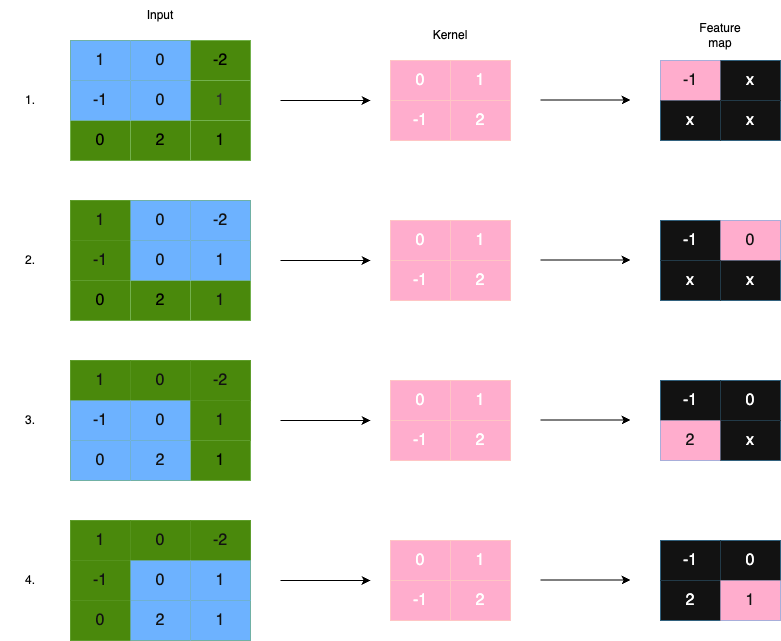
\includegraphics[width=0.8\textwidth]{Images/convolutional_operation.png}
  \caption{Illustration of the convolutional operation using a kernel on 2D input data.}
  \label{fig:convolution-diagram}
\end{figure}

\begin{definition}
  A \textit{Convolutional Neural Network (CNN)} \autocite{oshea2015introductionconvolutionalneuralnetworks} \autocite{jmse9040397} \autocite{LIU201711} is a discriminative deep learning model whose architecture is inspired by the hierarchical organization of the visual cortex in animals. CNNs are particularly effective in tasks involving image and spatial data processing due to their ability to capture local patterns and spatial hierarchies.

  The core components of a CNN are \textbf{convolutional layers} and \textbf{sub-sampling (pooling) layers}.

  \textbf{Convolutional layers} apply a set of learnable kernels (filters), each with its own weights, which slide over the input matrix to perform convolution operations. These layers extract local features by emphasizing patterns such as edges, textures, or more complex structures as the network deepens. They also preserve the spatial relationship between features, allowing the network to learn spatial hierarchies.

  \textbf{Sub-sampling layers}, also known as pooling layers, are used to progressively reduce the spatial dimensions of the feature maps. This helps decrease the computational complexity, control overfitting, and enhance the model’s invariance to small translations in the input. Common pooling operations include max pooling and average pooling, where the most prominent or average feature within a local region is retained. It's generally advised to use kernel size of 3 or less in pooling layers, due to their destructive nature and high chance of losing meaningful features.
\end{definition}

The concept of CNNs was inspired by Time-Delay Neural Networks, where weights are shared through time dimension. In CNNs weights are compacted into it's kernels. This architectural property vastly reduces the number of parameters and complexity of the network compared to Fully Connected Networks. CNNs are valued for their ability to learn to identify features without human interaction and for their empirically proven performance in processing multidimensional data with grid-like topology, like images and videos.

\section{Regularization}

\begin{definition}
  \textbf{Overfitting} \autocite{oshea2015introductionconvolutionalneuralnetworks} occurs when a model learns the details and noise in the training data to the extent that it negatively impacts the model’s performance on new, unseen data. This results in a model that has high accuracy on the training set but poor generalization to test data. Usually overfitting is indicated by model's performance on training dataset being much better then on test dataset \autocite{9944190}.
\end{definition}

Convolutional Neural Networks, despite their powerful feature extraction capabilities, are highly prone to overfitting (especially when trained on limited or imbalanced datasets) \autocite{alzubaidi2021review}. This is largely due to their large number of learnable parameters, which can easily adapt to noise in the training data. Regularization techniques are therefore essential to improve generalization and ensure that the model performs well on unseen data. Common methods include dropout, weight decay (L2 regularization), data augmentation, and early stopping. These techniques help constrain the learning process, reduce model complexity, and encourage the network to learn more robust and transferable features.

\begin{itemize}
  \item \textbf{Dropout:} \autocite{10.5555/2627435.2670313} A regularization technique where neurons are randomly deactivated during each training iteration. This prevents co-adaptation of neurons, encourages redundancy in feature learning, and improves generalization. During inference, the full network is used without dropout.

  \item \textbf{Data Augmentation:} \autocite{10.1145/3510413} Increases the size and diversity of the training dataset by applying transformations such as rotation, scaling, or flipping. This helps prevent overfitting and improves the model's ability to generalize.

  \item \textbf{Batch Normalization:} \autocite{NEURIPS2018_36072923} \autocite{10.1145/3510413} Normalizes layer outputs to have zero mean and unit variance. It reduces internal covariate shift, stabilizes training, and speeds up convergence by maintaining consistent activation distributions across training epochs. This normalization is applied to mini-batches during training and is often followed by a learnable scaling and shifting operation. By mitigating the shifting distributions of intermediate activations, batch normalization allows for higher learning rates, reduces sensitivity to initialization, and can also act as a form of regularization, sometimes reducing the need for dropout.

  \item \textbf{L1 and L2 Regularization:} \autocite{kukačka2017regularizationdeeplearningtaxonomy} These techniques add a penalty term to the loss function to discourage large weights and reduce the complexity of the model. L1 regularization (lasso) promotes sparsity by adding the absolute values of weights, and is represented by the term:
    \[
      \mathcal{L}_{L1} = \lambda \sum_{i} |w_i|
    \]
    where \( \lambda \) is the regularization strength and \( w_i \) are the model weights. L2 regularization (ridge) penalizes the squared values of weights, leading to smaller but non-zero weights, and is given by:
    \[
      \mathcal{L}_{L2} = \lambda \sum_{i} w_i^2
    \]
    The total loss function typically combines both the original loss and the regularization terms:
    \[
      \mathcal{L}_{total} = \mathcal{L}_{data} + \mathcal{L}_{L1} \text{ or } \mathcal{L}_{L2}
    \]
\end{itemize}

\section{Optimization}

\begin{definition}
  \textit{Gradient Descent} \autocite{sun2020optimization} \autocite{ruder2017overviewgradientdescentoptimization} is an iterative optimization algorithm used to minimize a loss function \( F(\theta) \) by updating the model parameters \( \theta \) in the direction of the negative gradient of the function. The basic update rule for gradient descent is given by
  \[
    \theta_{t+1} = \theta_t - \eta_t \nabla F(\theta_t),
  \]
  where \( \eta_t \) is the step size (also known as the learning rate), and \( \nabla F(\theta_t) \) is the gradient of the loss function evaluated at iteration \( t \).
\end{definition}

There are 3 variants \autocite{ruder2017overviewgradientdescentoptimization} of Gradient Descent: Batch Gradient Descent, Stochastic Gradient Descent and Mini-Batch Gradient Descent. Batch Gradient Descent Computes gradient for the whole dataset and performs the parameter update only afterwards.
% TODO: continue with other variants

\begin{definition}
  \textit{Backpropagation} \autocite{sun2020optimization} is an efficient algorithm for computing the gradient of the loss function with respect to the parameters of a neural network. Backpropagation systematically applies the chain rule of calculus layer by layer, propagating gradients backward from the output to the input to compute \( \nabla_\theta F_0(\theta) \) efficiently. From an optimization perspective, it enables the application of gradient-based methods, such as gradient descent, to train multi-layer networks.
\end{definition}

\begin{definition}
  \textit{Gradient Explosion/Vanishing} \autocite{sun2020optimization} refers to a common difficulty encountered when training deep neural networks, where gradients become either excessively large or exceedingly small as they are propagated backward through the network during training. From a signal processing perspective, gradient descent acts as a feedback correction mechanism: errors computed at the output layer are backpropagated through the network to update the weights of earlier layers. As this error signal passes through many layers, it may be repeatedly amplified (leading to gradient explosion) or attenuated (resulting in gradient vanishing). In either case, the learning process becomes unstable or stalls, preventing effective weight updates and model convergence.
\end{definition}

\begin{definition}
  \textit{Convergence} \autocite{sun2020optimization} in the context of optimization algorithms, particularly gradient descent, typically refers to the behavior where the sequence of iterates $\{\theta_t\}$ approaches a limit point as $t \rightarrow \infty$. A common formal criterion is that every limit point is a stationary point \autocite{bertsekas1997nonlinear}, meaning that the gradient vanishes at those points: $\nabla F(\theta^*) = 0$. However, this does not guarantee convergence to a global minimum and allows for several undesirable outcomes, such as the sequence having multiple limit points, or the sequence diverging with no limit points.
\end{definition}
\subsection{Optimization algorithms}
\subsection{Weights initialization}
% TODO: finish these sections

\chapter{Related Work}
\label{cha:RelatedWork}

\section{Previous Work at ScaDS.AI}

This thesis builds directly upon the foundational work conducted by König \autocite{konig2022model}, Flach \autocite{flach2023methods}, Schaller \autocite{schaller2023train}, and Schneeberger \autocite{schneeberger2024end}, continuing the exploration of autonomous driving agents in the field of machine learning. König's thesis is the earliest work among them. His focus was on training a model to navigate through an obstacle course composed of block-like barriers in a simulated setting. The structure of his obstacle course closely resembles the one used in this work, with a key distinction: the present thesis standardizes the obstacles by making them uniformly red and arranging them in pairs, which requires the vehicle to consistently pass between them, adding a layer of spatial precision to the navigation challenge.

König \autocite{konig2022model} employed a reinforcement learning methodology, specifically leveraging an evolution-based training approach. In contrast to the approach taken in this thesis, König \autocite{konig2022model} utilized an OpenCV-based image processing pipeline to identify obstacles and arena boundaries within the input images. These visual elements were then encoded into tensors that directly represented their spatial properties. As a result, there was no need for a Convolutional Neural Network (CNN), since the network was not required to extract spatial features from raw image data. Instead, a standard Artificial Neural Network (ANN) architecture was sufficient for his setup. His results demonstrated that the model successfully learned to handle a variety of generated obstacle configurations, showing a high degree of generalization across different courses. He concluded that the trained agent was capable of completing most of the parkour-style tracks effectively.

The work of Flach \autocite{flach2023methods} was a direct continuation of König’s earlier research \autocite{konig2022model}, with a focus on addressing one of the most significant challenges in autonomous agent development: bridging the Simulation-to-Reality (Sim2Real) gap. While König concentrated on training the agent within a controlled simulated environment, Flach aimed to transfer the trained model to a real-world setting. This step was crucial for validating whether behaviors learned in simulation could generalize effectively to physical environments. Flach \autocite{flach2023methods} used the same JetBot vehicle and physical arena that are also employed in the current thesis.

However, the transition to the real environment introduced several technical difficulties. One of the primary challenges was the difference in control dynamics between the simulated and physical JetBot vehicles, which made direct transfer of control strategies problematic. Additionally, Flach relied on an OpenCV-based visual processing pipeline, similar to König, which proved to be unreliable under varying real-world lighting conditions. The pipeline often misinterpreted background objects as obstacles and was particularly sensitive to brightness fluctuations, leading to inconsistent performance. The inability of the pipeline to detect object consistently has lead to the refuse to continue the research with the real world experiments and need in usage of the synthesized data. All these problems and differences have lead to the failure of transitioning the model from simulation to reality.

Schaller \autocite{schaller2023train} extended the research done by König \autocite{konig2022model} in addressing the main inaccuracies in his approach and the main problems that occurred during the Flach's \autocite{flach2023methods} research. His work addressed four central research questions, focusing on the feasibility of modeling autonomous driving as an RL problem, effective processing of camera input, overall learning performance, and the robustness of the algorithms under external influences. To achieve this, he developed four RL algorithms using carefully designed state representations and reward functions. These models demonstrated strong performance, particularly on easy and medium tracks, with the PPO-MEM-SGT algorithm even managing to complete the most challenging courses. Instead of using a convolutional neural network, Schaller \autocite{schaller2023train} extracted key coordinates from camera images to construct the state input, showing that simpler preprocessing can yield efficient results.

Schneeberger \autocite{schneeberger2024end} focused on developing a robust autonomous driving agent capable of adapting to varying lighting conditions. His approach employed an end-to-end trained Convolutional Neural Network (CNN), enabling the agent to directly learn control policies from raw visual input without relying on handcrafted feature extraction or preprocessing pipelines. The driving task was structured as a sequence of navigation goals across three difficulty levels, each presenting increasingly complex spatial configurations. The agent was evaluated under three distinct lighting conditions (bright, standard, and dark) designed to test its adaptability and generalization in diverse visual environments.

The results demonstrated that the CNN-based agent performed reliably across all difficulty levels and lighting settings, indicating a high degree of robustness and learning efficiency. By successfully addressing the limitations posed by inconsistent illumination (a challenge that had hindered earlier works) Schneeberger’s \autocite{schneeberger2024end} research marked a significant step forward in the development of more resilient autonomous driving systems.

\section{Imitation Learning}
The foundational paper on Imitation Learning is often credited to Pomerleau \autocite{NIPS1988_812b4ba2}. In this pioneering work, Pomerleau introduced a method for training a self-driving vehicle using a neural network that learns directly from human driving behavior. The approach, known as behavioral cloning, involved collecting image data from a forward-facing camera along with corresponding steering commands from a human driver. A neural network was then trained to map visual input to steering outputs, effectively imitating the demonstrated behavior. This paper laid the groundwork for the field of imitation learning by showing that autonomous control policies could be learned from demonstration rather than being manually programmed, opening the door to a range of data-driven approaches for robotics and autonomous systems.

The paper by Billard et al. \autocite{bakker1996robot} provides a comprehensive survey of imitation learning in the context of robotics, highlighting its potential as a natural and efficient framework for programming autonomous agents. The authors discuss key concepts, such as the distinction between mimicry and emulation, the challenges of mapping observed human actions to robot motor commands, and the importance of generalization beyond direct demonstrations. The paper categorizes imitation learning methods into different approaches, including behavioral cloning, inverse reinforcement learning, and correspondence mapping, offering insights into their strengths and limitations. By bridging insights from neuroscience, cognitive science, and machine learning, this work lays a conceptual foundation for designing robots that learn complex tasks by observing others, and it remains a seminal reference in the field.

\subsection{Imitation Learning Taxonomies}
Imitation Learning (IL) is traditionally categorized into two main approaches: Behavioral Cloning (BC) and Inverse Reinforcement Learning (IRL). Both branches have evolved by integrating diverse techniques and have been adapted to various application domains. Fundamentally, BC and IRL differ in how they aim to replicate expert behavior. BC typically learns a direct mapping from observed states to corresponding actions using supervised learning, whereas IRL focuses on inferring the underlying reward function that would make the expert's actions appear optimal. This fundamental distinction may explain why BC methods are more commonly deployed in real-world applications, while IRL remains largely confined to simulated environments, where the complexity and variability are easier to manage. \autocite{zheng2022imitationlearningprogresstaxonomies}

The definition of Behavioral Cloning (BC) was first proposed in \autocite{bain1995framework}. In this framework, BC is formulated as a supervised learning problem where the goal is to recover an expert policy $\pi_E$ from a set of demonstrations. Assume we observe a trajectory of state-action pairs ${(X_t, A_t)}_{0 \le t \le T}$, where the expert selects actions according to an unknown policy $\pi_E$, i.e., $A_t \sim \pi_E(\cdot \mid X_t)$. To imitate this behavior, we define a parametric policy class ${\pi\theta}_{\theta \in \mathbb{R}^d}$ and seek parameters $\theta$ that minimize a loss function between the learned policy and the expert’s observed behavior. A common approach is to minimize the empirical risk:
\[
  J_T(\pi_\theta) = \sum_{x \in \mathcal{X}} \sum_{a \in \mathcal{A}} \hat{\mu}_T(x) \left( \pi_\theta(a \mid x) - \hat{\pi}_{E,T}(a \mid x) \right)^2,
\]
where $\hat{\mu}_T(x) = \frac{1}{T+1} \sum_{t=0}^T \mathbb{I}_{\{X_t = x\}}$
are the empirical occupation frequencies under the expert’s policy, and $\hat{\pi}_{E,T}(a \mid x) = \frac{\sum_{t=0}^T \mathbb{I}\{X_t = x, A_t = a\}}{\sum_{t=0}^T \mathbb{I}\{X_t = x\}}$ is the estimate of expert policy. \autocite{neu2012apprenticeshiplearningusinginverse}

A formal definition of Inverse Reinforcement Learning was first introduced by Russell \autocite{russell1998learning}. In this formulation, the objective is to infer the underlying reward function that an expert is implicitly optimizing, based solely on observations of their behavior. Unlike standard reinforcement learning, where the reward function is known and the goal is to learn a policy, IRL reverses this process by assuming access to expert trajectories and attempting to deduce the reward structure that would make such behavior optimal. This approach is particularly useful in scenarios where specifying a reward function manually is difficult or unintuitive, such as in complex human tasks. Russell’s work laid the theoretical groundwork for a wide range of subsequent research, leading to more advanced IRL algorithms that are now used in robotics, autonomous systems, and human behavior modeling.

Imitation Learning (IL) can also be classified into model-based and model-free approaches, depending on whether the algorithm utilizes a forward model to understand environmental dynamics. In model-based methods, the agent attempts to learn or leverage a model of how the environment responds to actions, while model-free methods bypass this by learning policies directly from data. Historically, most IRL (Inverse Reinforcement Learning) methods have been model-based, as they often require iterative evaluations within the environment to infer the underlying reward function. In contrast, Behavioral Cloning (BC) methods are typically model-free, since they rely on supervised learning and often assume access to a low-level controller. The introduction of Generative Adversarial Imitation Learning (GAIL) \autocite{ho2016generative} marked a shift, enabling IRL-style imitation in a model-free setting. This led to the development of various adversarially structured IL algorithms that follow GAIL’s paradigm.

While incorporating a model of the environment can provide richer contextual information and improve data efficiency, it is not always necessary—or even feasible—depending on the task. Model learning can be both computationally expensive and technically challenging. In domains like robotics, where precise measurements such as position and velocity are easily accessible, the benefits of modeling system dynamics may be minimal. However, in complex scenarios such as autonomous driving, understanding dynamics can be essential for safety, such as avoiding collisions with pedestrians. Ultimately, the choice between model-based and model-free approaches should be guided by the specific demands and constraints of the application. \autocite{zheng2022imitationlearningprogresstaxonomies}

\section{Imitation Learning in Autonomous Driving}

\subsection{Behavioral Cloning}

As mentioned earlier, Imitation Learning in autonomous driving traces its roots back to the late 1980s with pioneering projects like Autonomous Land Vehicle In a Neural Network (ALVINN) \autocite{NIPS1988_812b4ba2}. ALVINN was one of the first systems to apply neural networks to autonomous navigation by training a vehicle to mimic human driving behavior. It used a single-layer neural network to map input from a forward-facing camera and a laser rangefinder directly to steering commands. The model was trained using supervised learning from human driving demonstrations, making it an early form of Behavioral Cloning. Despite the limited computational resources of the time, ALVINN successfully drove a van on public roads for extended distances, showcasing the feasibility of learning-based control systems.

One of the biggest works in application of Behavioral Cloning to autonomous driving was the DAVE project \autocite{muller2004autonomous}, developed in the Defense Advanced Research Projects Agency (DARPA). This early system demonstrated that it was possible to train a neural network to control a vehicle by learning from a dataset that contains only data collected by the camera. They used 2 cameras to collect the images from different perspectives, so that despite not having any other sensors installed on the vehicle, the model would have been able to learn to estimate the depth. As a result they've captured a slightly better performance from the model trained and executed using a binocular setup, rather than the monocular one.

Building on the foundations of DAVE, NVIDIA introduced its own successor, DAVE-2 \autocite{bojarski2016endendlearningselfdriving}, which represented a significant leap forward in autonomous driving research. DAVE-2 utilized a deep Convolutional Neural Network trained entirely using Behavioral Cloning. By processing raw pixel data from front-facing cameras, the network could learn to output steering angles, demonstrating impressive lane-following capabilities in real-world environments. The CNN architecture of many other works about autonomous driving was inspired by DAVE-2. List of such works includes the paper from Farag et al. \autocite{8855753}, on which this thesis was mostly based on and whose architecture was used (with certain adjustments) for the CNN architecture in this work. The idea of using the LSTM layers \autocite{6795963} was also inspired by the "Future work" section of this paper.

In addition to DAVE-2, NVIDIA also developed PilotNet, which became their first autonomous driving system capable of navigating highways with minimal human intervention. They've utilized a much more sophisticated CNN architecture, which includes residual \autocite{he2015deepresiduallearningimage}, convolutional and fully connected layers. In contradiction to previous autonomous systems, PilotNet's output is not just a steering angle, but rather a driving trajectory. The reasoning behind using this approach is that the steering angle doesn't fully represent the decision-making process of the car driver, which in it's turn is dictated by the car's geometry, slope and obstacles on the road. PilotNet was designed to produce the three-dimensional trajectory, that would then be fed into an independent controller guiding the car along it. Like its predecessors, PilotNet followed an end-to-end learning paradigm, relying on supervised learning from human drivers. This system marked a practical transition from research prototypes to road-capable AI systems, showcasing the effectiveness of Behavioral Cloning for structured environments such as highways.

\subsection{Model Predictive Control}

Model Predictive Control (MPC) is an advanced control strategy that optimizes control inputs by predicting future system behavior over a finite time horizon. At each time step, MPC solves an optimization problem to minimize a cost function subject to system dynamics and constraints, implementing only the first control input and repeating the process at the next time step.

The most effective MPC algorithm for autonomous driving known to date is Model Predictive Path Integral (MPPI) Control \autocite{williams2017model} \autocite{kappen2005linear}. MPPI is a stochastic optimal control method derived from the path integral formulation of control. It computes control actions by evaluating the expected cost of a large number of sampled control sequences under system dynamics. Given a nonlinear system with state \(\mathbf{x} \in \mathbb{R}^n\) and control \(\mathbf{u} \in \mathbb{R}^m\), the algorithm samples trajectories \(\{\mathbf{u}_k^{(i)}\}_{i=1}^N\) around a nominal control sequence \(\{\bar{\mathbf{u}}_k\}_{k=0}^{T-1}\), where \(N\) is the number of trajectories and \(T\) is the time horizon. The cost associated with each trajectory is computed as:

\[
  S^{(i)} = \sum_{k=0}^{T-1} q(\mathbf{x}_k^{(i)}, \mathbf{u}_k^{(i)}) + q_T(\mathbf{x}_T^{(i)}),
\]

where \(q(\cdot)\) and \(q_T(\cdot)\) denote the running and terminal cost functions, respectively.

In the work by Williams et al. \autocite{williams2016aggressive} they've used a cost function based on the vehicle's position relative to the lane. Despite the simplicity of the cost function, they were able to obtain results when the system is able to operate on a very high velocity.

The cost function can also be replaced replaced by a neural network, as in \autocite{drews2017aggressivedeepdrivingmodel}. Here they've developed a CNN that would output the cost function based on the image from the frontal camera. They've tested two approaches: in the first one the cost map was directly derived from the image and it was dependent on the camera angle. In the second approach they focused on generating the cost map from the top view. The second approach has shown to be more effective in both training evaluation and test experiments.

In the work by Pan et al. \autocite{pan2019agileautonomousdrivingusing} the authors used MPPI algorithm as an expert for collecting the demonstrations in both real and virtual environment. The CNN was used to learn from these demonstrations. They've used DAgger methodology \autocite{ross2011reduction} to collect more data by gradually increasing the impact of the CNN part in the demonstrations with each iteration.


\chapter{Behavioral Cloning for Autonomous Driving through the Obstacle Course}
\label{cha:Main}

\section{Environment Setup}

\subsection{Arena}

The arena used in this thesis is represented as a \(2 \times 1\) meter surface, on which obstacles measuring \(4 \times 4 \times 16\) cm are placed. The setup resembles the one used in König’s thesis \autocite{konig2022model}, with the key difference being that all obstacles in the current thesis are of a single color. To ensure measurement precision as well as material stability and robustness, 3D-printing technology was chosen for obstacle fabrication. This approach also facilitates a smooth transition to virtual reality, in case virtualization becomes necessary.

To address the first difficulty, the obstacles were glued to the arena surface to ensure they maintained their exact positions during preparation and evaluation. However, for the second difficulty (where frequent repositioning of obstacles is required) they were left unglued. In each experimental run, three pairs of obstacles are installed on the arena. Their positions are deliberately selected to maximize the likelihood that they remain within the camera’s field of view until the robot passes them.

\subsection{Hardware}

To collect training data and evaluate the trained models, the NVIDIA JetBot is employed, consistent with previous research conducted by ScaDS.AI. The JetBot is powered by a Jetson Nano module, which features 4 GB of LPDDR4 memory and 128 CUDA cores, capable of running at a maximum clock speed of 921 MHz. These computational capabilities are sufficient to execute the entire control inference pipeline at a frequency of 4 Hz, ensuring timely responses for real-time navigation tasks. The detailed description of the pipeline is represented in \autoref{sec:pipeline}.

The movement system consists of two DC motors with integrated encoders, connected to the Jetson Nano through a motor driver interface. This allows the control of the robot’s differential drive mechanism, enabling it to perform turns and controlled straight motion. The motors are powered by a rechargeable lithium-ion battery, providing enough energy for several hours of operation under typical loads.

For motor control and overall robot management, the JetBot API was used, which conveniently provides \texttt{Python} bindings. This allows integration with the data acquisition and inference components, all of which are written in \texttt{Python}. Although the API includes various methods to control the JetBot, this thesis adopts the direct velocity control method. For each of the two motors the velocity can be set to any value within the range \([-1, 1]\), where \(-1\) corresponds to full reverse, \(0\) to a stationary motor, and \(1\) to full forward speed. This approach simplifies the control logic and makes the task of mapping the joystick inputs to control signals more straightforward.

Additional peripherals include a wide-angle Raspberry Pi Camera BMP (V2) module, used for visual input, and a Wi-Fi module for remote access and debugging. The camera captures frames at a resolution suitable for both training and real-time inference with the maximum frame rate of 120 Hz.

\subsection{Software}

To facilitate frequent modifications to the model architecture, the \texttt{Keras} framework was chosen for development. \texttt{Keras} is a high-level neural network API for \texttt{Python} programming language built on top of \texttt{TensorFlow}, which handles GPU acceleration, memory management, and other low-level operations. This abstraction significantly simplifies the design and training of deep learning models. The primary motivations for selecting \texttt{Keras} include its intuitive syntax, extensive library of pre-built layers, activation functions, loss functions, and optimizers, as well as its strong community support and documentation.

\texttt{Keras} also includes a convenient toolkit for training workflows, featuring integrated support for image data preprocessing and augmentation. However, since this thesis involves working with temporal sequences of image frames, which requires accurate frame rate consistency for the training, a custom data augmentation pipeline was implemented. This custom solution ensures that temporal integrity is maintained when transforming image sequences during training, which is critical for models that rely on time-dependent input data.

During development, version compatibility issues were encountered, particularly with \texttt{TensorFlow} on the Jetson Nano hardware. The Jetson platform supports only specific versions of cuDNN, a prerequisite for GPU-accelerated \texttt{TensorFlow}. Consequently, it was necessary to downgrade \texttt{TensorFlow} to a compatible version across the entire project to maintain consistency between training and experimental environments.

For numerical operations, the \texttt{NumPy} library was employed. \texttt{NumPy} provides a rich collection of mathematical functions that are implemented in optimized \texttt{C/C++} code. This enables efficient numerical computation in \texttt{Python}, which is essential for tasks such as preprocessing datasets, manipulating input tensors, and analyzing model outputs.

All image processing tasks, including resizing, cropping, filtering, and saving frames, were performed using the \texttt{OpenCV} library. \texttt{OpenCV} offers an extensive suite of image manipulation functions and is highly optimized for real-time performance. It proved indispensable throughout the development process, particularly during data collection, visualization, and debugging phases.

\section{Data Acquisition}

To perform supervised learning using Behavioral Cloning, it was necessary to collect a labeled dataset. The dataset \( D \) is represented as a sequence of input-output pairs \( (x_i, y_i) \in D \), where \( x_i \) denotes the sensor input (in this case, camera frames), and \( y_i \) represents the corresponding control signal required for the robot at that point in time. To generate these labels, a gamepad was used, with the inclination of its left analog stick mapped to motor speed values for the JetBot using a special function.

To streamline the data collection process, a custom data acquisition pipeline was developed. Its primary goals were to (1) allow real-time control of the JetBot via the gamepad, (2) capture synchronized sensor data, and (3) store the collected data in a structured format. The pipeline consists of two components:

\begin{itemize}
  \item \textbf{Server}: runs on the JetBot and handles both motor control and video capture.
  \item \textbf{Client}: runs on an external machine connected to the same local network, responsible for reading gamepad inputs and sending them to the server.
\end{itemize}

The pipeline operates as follows:

\begin{enumerate}
  \item The server program is launched on the JetBot. It spawns two concurrent threads:
    \begin{itemize}
      \item One thread initializes the OpenCV video capture pipeline to continuously collect frames from the onboard camera.
      \item The second thread starts a TCP server using \texttt{Python}’s built-in \texttt{socket} library, listening for incoming connections on a designated port.
    \end{itemize}

  \item The client program is executed on another machine. It verifies the presence of a connected gamepad and begins listening for control inputs using the \texttt{pygame} library, which provides low-level access to hardware devices.

  \item Once a connection is established, the client begins transmitting the current position of the gamepad’s left analog stick to the JetBot server.

  \item The TCP server thread on the JetBot receives the input data and updates a shared variable, which is accessed by the video thread.

  \item When a new video frame is captured, it is stored locally. Simultaneously, the server retrieves the most recent gamepad input from the shared variable and calculates the corresponding motor speeds. For an analog stick input represented as \( (x, y) \), the left and right motor speeds are derived using the calculations described in Algorithm \ref{alg:motor_inputs}.

  \item The computed motor commands are then sent to the JetBot’s motors via the JetBot API, and the process repeats in real time until manual termination.

  \item Upon termination, the collected data is transferred from the JetBot to the client machine. All captured video frames are stored in a dedicated directory as image files, while the control sequence is saved in the same directory using NumPy's binary format (\texttt{.npy}). Each control entry is stored as a tuple \( (x, y, t) \), where \( x \) and \( y \) are the analog stick positions, and \( t \) is the timestamp in milliseconds from the start of the recording session.
\end{enumerate}

\begin{algorithm}
  \caption{Calculation of motor inputs based on the gamepad's stick position}
  \begin{algorithmic}[1]
    \Function{CalculateMotorInputs}{$x, y$}
    \State $\text{rotation\_quotient} \gets 0.5$
    \State $left\_power \gets -y + x \cdot \text{rotation\_quotient}$
    \State $right\_power \gets -y - x \cdot \text{rotation\_quotient}$
    \State $max\_power \gets \max\left( \left|left\_power\right|, \left|right\_power\right|, 1 \right)$
    \State $left\_power \gets left\_power / max\_power$
    \State $right\_power \gets right\_power / max\_power$
    \State \Return $left\_power, right\_power$
    \EndFunction
  \end{algorithmic}
  \label{alg:motor_inputs}
\end{algorithm}

The data was initially collected at a frame rate of 30 frames per second (FPS). However, it was later decided to increase the frame rate to 120 FPS, as it is the fastest framerate that the sensor can provide. The rationale behind this decision was that, although the system is not capable of executing the control policy at such a high frequency in real-time, the high-frame-rate sequences could be downsampled during training using time and frequency warping techniques \autocite{iglesias2023data}. This allows for greater flexibility in choosing the effective temporal resolution for training, depending on the model architecture and experimental requirements.

After data collection, a filtering step was applied to remove unrepresentative or low-quality trajectories. In particular, sequences that did not contribute meaningful information to the learning process (such as those recorded after the JetBot had passed the final obstacle pair) were discarded entirely. Additionally, some valid trajectories were cropped to eliminate irrelevant frames that might hinder effective feature extraction during training.

The final dataset consists of 22,017 labeled images and is divided into two subsets: one for the first difficulty level and the other for the second difficulty level. The first difficulty subset contains 15,008 data points, while the remaining 7,009 correspond to the second difficulty.

It is important to note that the quality and quantity of data for the second difficulty level are suboptimal. Compared to the first difficulty, the second requires a significantly higher degree of generalization from the model due to increased environmental variability. Ideally, the dataset for the second difficulty would have included more examples with greater diversity and a broader distribution of features. However, due to time constraints, the substantial workload involved in completing this thesis, and the labor-intensive nature of data acquisition and filtering, it was decided to proceed with training using the existing dataset.

\section{Data Pre-processing}

Before initiating the training process, the collected data must be pre-processed to enhance training efficiency and reduce the impact of irrelevant noise that could impair the model's ability to learn meaningful features. The pre-processing steps applied to the images and used in the final training iteration are illustrated in \autoref{fig:preprocessing} and outlined below:

\begin{enumerate}
  \item \textbf{Grayscale Conversion} \\
    Due to hardware limitations in terms of memory and computational resources on the JetBot platform, the model must be lightweight and capable of making inferences in real time. To reduce computational complexity and model size, all images are converted to grayscale prior to being fed into the neural network. This eliminates color information while preserving structural features necessary for decision-making. The grayscale transformation is performed using the standard luminance-preserving formula:
    \[
      Y = 0.299 \times R + 0.587 \times G + 0.114 \times B
    \]
    where \( R \), \( G \), and \( B \) denote the red, green, and blue color channels, respectively.

  \item \textbf{Region of Interest (ROI) Cropping} \\
    To further reduce the computational load and focus the model’s attention on the most relevant parts of the input, a region of interest is cropped from each image. This not only reduces the input dimensionality (thereby speeding up both training and inference), but also increases the proportion of informative pixels that are likely to contribute to effective feature extraction.

  \item \textbf{Pixel Centering} \\
    Convolutional Neural Networks (CNNs) typically benefit from normalized input data. As shown in prior research \autocite{pal2016preprocessing}, normalization helps accelerate convergence and improve model performance. In the final model implementation, all grayscale images are centered around zero by applying the following normalization:
    \[
      Y_c = \frac{Y}{127.5} - 1
    \]
    where \( Y \) is the grayscale image matrix and \( Y_c \) is the normalized output passed to the network.

    Z-score normalization approach was also experimented on, but it didn't show any better results compared to the pixel-centered approach.

  \item \textbf{Update memory stack} \\
    Once the image is passed through all of the preprocessing steps, the memory stack of size $N$ is updated by pushing the frame to its top position. The stack size $N$ is usually set to $10$ after hyperparameter tuning that yielded the best parameters with which the model has the best training results.
\end{enumerate}

\begin{figure}[htbp]
  \centering
  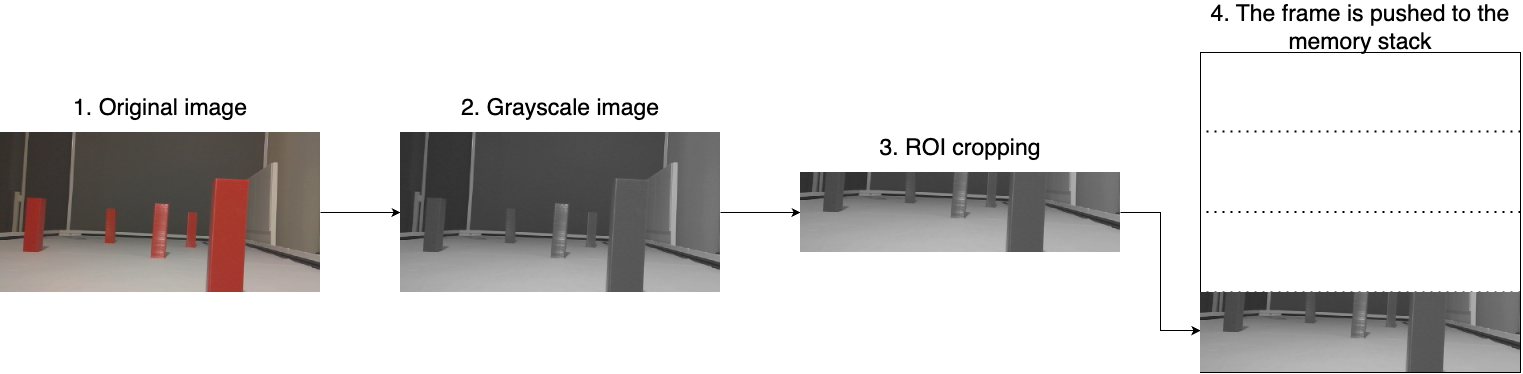
\includegraphics[width=0.9\textwidth]{Images/preprocessing.png}
  \caption{Input preprocessing pipeline.}
  \label{fig:preprocessing}
\end{figure}

\subsection{Edge Detection}
\label{sec:edge-detection}

Although the final version of the control inference system utilizes relatively simple and direct pre-processing steps, a substantial amount of experimentation was conducted to evaluate other more advanced techniques and determine the most effective configuration.

One such technique, proposed as a direction for future work by Farag et al. \autocite{8855753}, is the application of edge detection to input images prior to processing by a Convolutional Neural Network (CNN). The intuition behind this method is that edge detection enhances object boundaries, potentially making it easier for a CNN to extract meaningful features from the input. This, in theory, could simplify the task of identifying obstacles and accelerate the model’s ability to learn complex and task-relevant visual patterns.

To test this hypothesis, two well-known edge detection algorithms were evaluated: the Canny edge detector \autocite{canny1986computational}, as recommended by Farag et al. \autocite{8855753}, and the Sobel filter \autocite{sobel2014history}. These approaches were selected, because after testing multiple edge detection algorithms, they seemed to produce the most meaningful and noiseless outputs. Models were trained using data processed by each of these algorithms. However, empirical results showed no significant improvements in performance or generalization capability. The best outcome achieved with edge-detected inputs was that the JetBot was able to consistently pass the second pair of obstacles but failed to navigate the third.

\begin{figure}[htbp]
  \centering
  \tabulinesep=1.2mm
  \begin{tabu}{cc}
    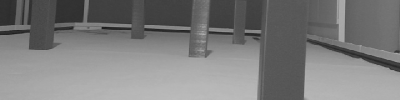
\includegraphics[width=0.4\textwidth]{Images/EdgeDetection/original.png} & 
\includegraphics[width=0.4\textwidth]{Images/EdgeDetection/blurred.png} \\
    \parbox{0.4\textwidth}{\centering (a) Original grayscale image.} &
    \parbox{0.4\textwidth}{\centering (b) Gaussian Blur is used to remove the noise before applying edge detection.} \\
    
\includegraphics[width=0.4\textwidth]{Images/EdgeDetection/canny_edges.png} & 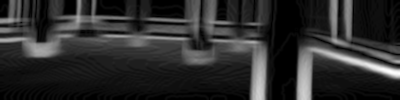
\includegraphics[width=0.4\textwidth]{Images/EdgeDetection/sobel_edges.png} \\
    \parbox{0.4\textwidth}{\centering (c) Canny edge detection algorithm.} &
    \parbox{0.4\textwidth}{\centering (d) Sobel filter applied to the image in $x$ and $y$ directions.} \\
    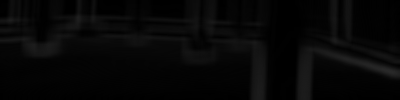
\includegraphics[width=0.4\textwidth]{Images/EdgeDetection/morphological_edges.png} & 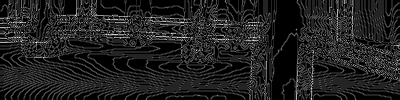
\includegraphics[width=0.4\textwidth]{Images/EdgeDetection/log_edges.png} \\
    \parbox{0.4\textwidth}{\centering (e) Morphological gradient operation for edge enhancement.} &
    \parbox{0.4\textwidth}{\centering (f) Laplacian of Gaussian (LoG) edge detection.} \\
  \end{tabu}
  \caption{Examples of the output of different edge detection algorithms.}
\end{figure}

In contrast, the baseline model trained on unprocessed grayscale images exhibited significantly better performance. The poor results with edge-detected inputs are likely due to the sensitivity of these algorithms to noise. Although Gaussian blurring was applied to smooth the images and reduce noise, both Canny and Sobel methods still introduced visual artifacts that the model may have incorrectly interpreted as important features.

While edge detection remains a conceptually promising technique, it did not yield practical benefits in the context of this project. An additional idea explored was the use of Quantized Neural Networks (QNNs), in which network weights are represented as low-precision integers or even binary values. Given that the Canny edge detector produces binary output, it would be theoretically feasible to design a quantized CNN specifically tailored to such input. This approach could significantly reduce model size and enhance computational efficiency, as integer operations are less resource-intensive than floating-point calculations. However, due to time constraints and the lack of observed performance gains from edge detection, this prospect was not pursued further in this work.

\section{Model Architecture}

One of the primary objectives of this thesis was to design a Convolutional Neural Network (CNN) architecture capable of effectively learning and extracting relevant features from image sequences. As in previous works, the model would need to capture not only spatial features from individual frames but also temporal dependencies across a sequence of images. This requirement necessitated the incorporation of a memory mechanism, as introduced in prior works such as \autocite{schneeberger2024end} and \autocite{schaller2023train}.

To identify the most suitable model architecture for the task, various configurations and design strategies were explored. Dozens of architectures were implemented and evaluated, with many discarded early due to poor performance. Below is a summary of some of the architectures that were tested on the way of reaching the satisfactory results:

\begin{enumerate}
  \item \textbf{Previous Thesis-Based Approach:} \\
    The architectures proposed by Schneeberger \autocite{schneeberger2024end} and Schaller \autocite{schaller2023train} processed the input image sequence using multiple convolutional channels --- one per image. To replicate this design, the CNN model from OpenAI’s Stable Baselines 3, originally implemented in \texttt{PyTorch}, was reimplemented in \texttt{Keras} and adjusted to conform to dimensional requirements. The architectural layout is shown in \autoref{fig:sb3cnn-arch}.

    \begin{figure}[htbp]
      \centering
      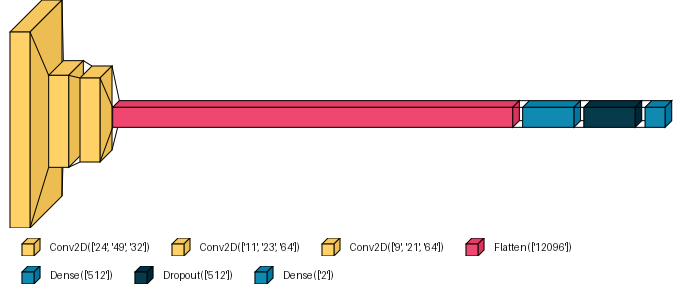
\includegraphics[width=0.8\textwidth]{Images/SB3CNN_architecture.png}
      \caption{Architecture diagram of the CNN model from Stable Baselines 3.}
      \label{fig:sb3cnn-arch}
    \end{figure}

    This model didn't show the ability to learn from the given dataset, most likely due to it being too shallow to be able to capture meaningful features from high-dimensional inputs. The validation loss sank early, causing the Early Stopping mechanism to terminate training at epoch 10.

  \item \textbf{DAVE-2:} \\
    This architecture, originally developed by NVIDIA researchers \autocite{bojarski2016endendlearningselfdriving}, was replicated exactly as described in the original publication. It is the only model evaluated in this thesis that does not incorporate any memory mechanism and also does not require preprocessing beyond simple image cropping. The network accepts raw RGB images as input using a 3-channel input layer and is visualized in \autoref{fig:dave-2-arch}.

    \begin{figure}[htbp]
      \centering
      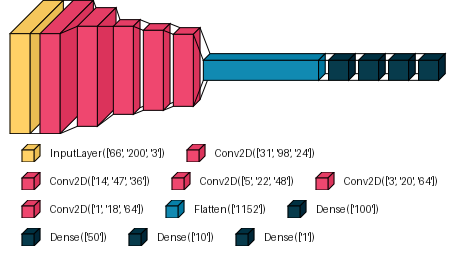
\includegraphics[width=0.5\textwidth]{Images/DAVE-2_architecture.png}
      \caption{DAVE-2 architecture.}
      \label{fig:dave-2-arch}
    \end{figure}

  \item \textbf{BCNet with LSTM:} \\
    BCNet, proposed by Farag et al. \autocite{8855753}, shares structural similarities with DAVE-2 but includes key differences such as the number and sizes of layers. While originally designed to predict the vehicle’s steering angle, the model was adapted for this thesis to conform to the task of predicting the velocity of the motors.

    In their work, Farag et al. also proposed several potential improvements, including the integration of Long Short-Term Memory (LSTM) layers and the use of edge detection during preprocessing. As discussed in \autoref{sec:edge-detection}, edge detection did not yield beneficial results in this context. However, the integration of LSTM layers was implemented to capture temporal patterns in the image sequence.

    Both LSTM and convolutional LSTM layers were planned to be experimented on. However, since the \texttt{cuDNN} version installed on the JetBot is not the latest, some CUDA API features that are required to use \texttt{Keras}’s \texttt{ConvLSTM2D} with GPU acceleration are not available. For this reason only casual convolutional LSTM layers were utilized to implement the architecture design of the model.

    The resulting architecture is illustrated in \autoref{fig:BCNet-LSTM-arch}. To integrate the LSTM component, \texttt{Keras}’s \texttt{TimeDistributed} layers were employed. These layers apply convolutional operations to each frame in the sequence independently, enabling the sequential outputs to be passed collectively to the LSTM block for temporal processing.

    \begin{figure}[htbp]
      \centering
      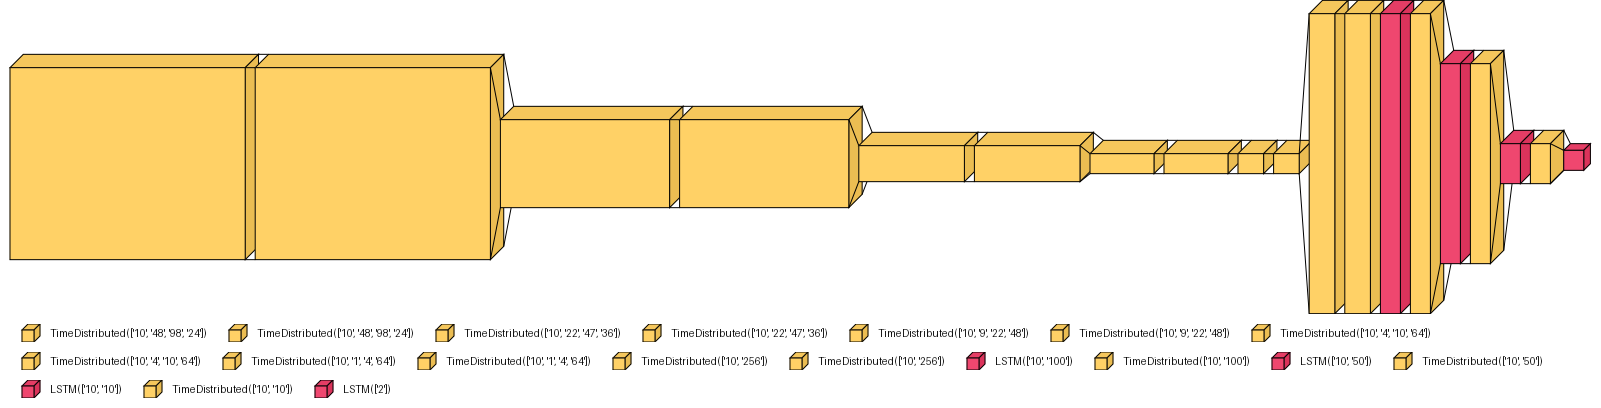
\includegraphics[width=1.0\textwidth]{Images/BCNetLSTM_architecture.png}
      \caption{BCNet with LSTM layers. The \texttt{TimeDistributed} layers represent convolutional, flattening, and dropout operations across the sequence.}
      \label{fig:BCNet-LSTM-arch}
    \end{figure}
\end{enumerate}

\section{Training Process}

The training process for the models involves multiple stages, including data preprocessing, dynamic batching, augmentation, and iterative refinement of model hyperparameters. Due to the constraints of hardware resources, the training pipeline must be both efficient and robust. One of the main components enabling this is the data generator, which is responsible for assembling input sequences and labels on the fly, thereby allowing for large-scale training without exceeding system memory limits.

\subsection{Data Generator}

Given the size of the dataset, which exceeds the available Random Access Memory (RAM) on most devices, a dynamic data generator is implemented. Its primary function is to generate training data sequences incrementally, processing and yielding data batch by batch during training.

The generator constructs temporal sequences of input frames, ensuring that the interval between consecutive frames in each sequence is not shorter than the minimum time interval required by the control inference pipeline to operate effectively. This interval is determined based on timestamp differences stored in the dataset. If a particular frame is the first in a trajectory and lacks any predecessors, the memory stack is padded with zero-valued matrices to account for the missing historical context.

For training, a maximum frame frequency of 4 Hz is typically used. This rate provides a balance between temporal resolution and computational load and is sufficient for most models to make their predictions, particularly when controlling the JetBot at low velocities.

After all frames are pre-processed and collected into the memory stack, a corresponding label must be generated for the data sequence. The label is obtained from the coordinates of the joystick's left analog stick in the frame immediately following the last frame in the sequence. Several alternative strategies were explored, including predicting the joystick position of the current frame or of a frame two steps ahead. However, predicting the next frame's joystick position yielded the best results. This can be explained by the latency of the inference pipeline: the system requires approximately $\frac{1}{4}$ seconds to compute the motor commands and invoke the API to apply them. In the case the model requires less time for the prediction, the pipeline is artificially slowed down to conform the target frequency. By the time this process is complete, the system's state has already changed. Therefore, predicting the immediate future state (i.e., the next frame) aligns more closely with real-world control requirements.

An alternative approach was also evaluated, where the labels consisted of direct motor velocity signals rather than joystick coordinates. This method is inspired by the research of Hwangbo et al. \autocite{hwangbo2019learning}, who reported improved performance when training legged robots using low-level actuator signals. However, in experiments run on the JetBot, using motor velocities as labels led to significantly worse model performance compared to using analog stick coordinates. This difference is likely due to differences in robot construction (legged vs. wheeled), training methodologies, and experimental setups.

Once the state-label pair is assembled, it is stored in a buffer array used for data augmentation. The number of stored instances is determined by a user-defined parameter passed to the data generator. During subsequent iterations, with a certain probability, the generator may retrieve a stored pair from the augmentation buffer, apply a set of transformations (see \autoref{sec:augmentation}), and yield the augmented data before proceeding with the next unmodified pair.

If the data generator completes an iteration over all data points within a given subset of the dataset and entries remain in the augmentation buffer, it proceeds to process each of these stored entries. This stochastic sampling logic ensures that transformed pairs are not immediately following their original counterparts. Moreover, this approach guarantees that each data point is replicated and transformed precisely the number of times specified by the user-defined augmentation parameter.

The step-by-step description of the data generator is described in the Algorithm \ref{alg:data_generator}.

\subsection{Data Augmentation}
\label{sec:augmentation}

Data augmentation is a well-established strategy for improving model generalization, especially in cases where collecting large, diverse datasets is infeasible. In the context of time series data, augmentation methods can be particularly impactful, since transformations applied by them can modify not only spatial, but also temporal structures of the data \autocite{iglesias2023data}.

This work adopts a hybrid augmentation strategy that applies both temporal and spacial transformations to the training data. For the temporal component, \textbf{time warping} is implemented by dynamically adjusting the maximum allowed frame frequency \( f_{\text{max}} \) for data pairs retrieved from the augmentation buffer. By increasing or decreasing the time between frames in a sequence, the generator effectively simulates variations in system response time or actuation speed, thus improving the model's robustness to timing deviations.

Spacial transformations are also applied to the augmented input data. They're applied probabilistically and independently to each image in the memory stack:

\begin{itemize}
  \item \textbf{Gaussian Noise Injection (Jittering):} Gaussian noise with a random standard deviation \( \sigma \in [0, 0.5] \) is added to simulate sensor noise or varying lighting conditions.
  \item \textbf{Translation:} The image is randomly shifted along both axes within a maximum offset of 9 pixels, simulating minor misalignments or camera movement.
  \item \textbf{Rotation and Scaling:} A small random rotation (up to \( \pm 5^\circ \)) and scaling (within \( \pm 6\% \)) are applied using affine transformations. This accounts for slight perspective distortions and variations in camera zoom.
\end{itemize}

\begin{figure}[htbp]
  \centering
  \begin{tabu}{cc}
    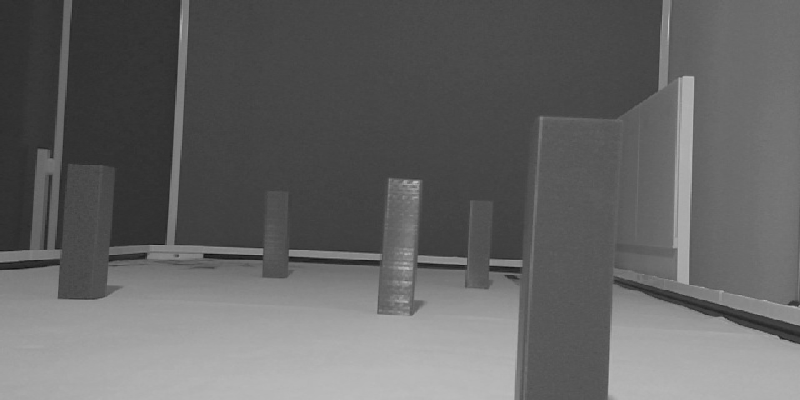
\includegraphics[width=0.4\textwidth]{Images/Augmentation/original.png} & 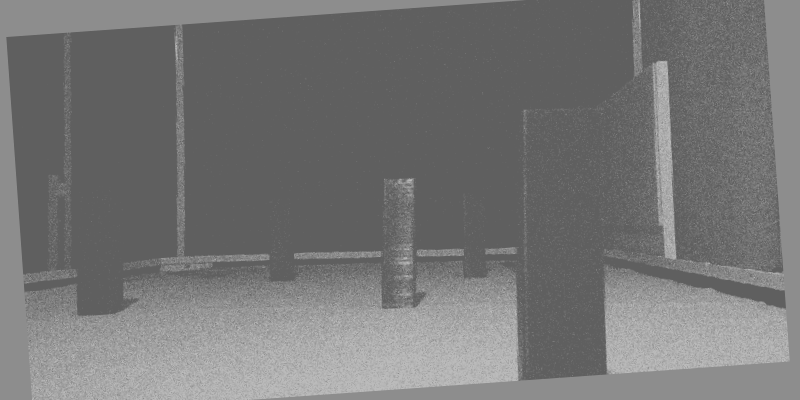
\includegraphics[width=0.4\textwidth]{Images/Augmentation/transformed.png} \\
    \parbox{0.4\textwidth}{\centering (a) Original image.} &
    \parbox{0.4\textwidth}{\centering (b) Transformed image.}
  \end{tabu}
  \caption{Example of an image being transformed in the result of data augmentation.}
  \label{fig:augmentation_transformations}
\end{figure}

The augmentation process is applied during data generation, immediately before yielding the augmented state-label pair. This ensures that transformations are computed on-the-fly and vary across training epochs, further reducing the risk of overfitting.

By combining time series augmentation principles, as outlined in \autocite{iglesias2023data}, with low-level image manipulation techniques, the data generator enhances both temporal and spacial diversity in the training dataset. This dual-augmentation approach has shown to significantly improve the stability and adaptability of the resulting control model.

\begin{algorithm}[H]
  \caption{Data Generator for Incremental Training with Augmentation}
  \begin{algorithmic}[1]
    \Require Dataset $D$, max frame frequency $f_{max} = 4$ Hz, memory stack size $N$, augmentation factor $k$, augmentation probability $p$
    \Ensure Yields $(state, label)$ pairs for training

    \State Initialize augmentation buffer $A \gets \emptyset$
    \ForAll{data points $d_i \in D$}
    \State Initialize memory stack $M_i \gets \emptyset$
    \State Set current index $j \gets i$
    \While{$|M_i| < N$ and $timestamp(d_j) > 0$}
    \If{$timestamp(d_j) - timestamp(d_{j-1}) \geq \frac{1}{f_{max}}$}
    \State Append $d_j$ to $M_i$
    \EndIf
    \State $j \gets j - 1$
    \EndWhile
    \If{length of $M_i < N$}
    \State Pad $M_i$ with zero-matrices until size $N$
    \EndIf
    \State Extract label $y_i$ from $d_{i+1}$
    \State Store $(M_i, y_i)$ in $A$ $k$ times based on augmentation factor
    \If{random() $< p$ and $A \neq \emptyset$}
    \State Select random $(M_j, y_j)$ from $A$
    \State Apply augmentation to $(M_j, y_j)$ to get $(\hat{M}_j, \hat{y}_j)$
    \State \textbf{yield} $(\hat{M}_j, \hat{y}_j)$
    \EndIf
    \State \textbf{yield} $(M_i, y_i)$
    \EndFor
    \If{$A \neq \emptyset$}
    \ForAll{$(M_j, y_j) \in A$}
    \State Apply augmentation to $(M_j, y_j)$ to get $(\hat{M}_j, \hat{y}_j)$
    \State \textbf{yield} $(\hat{M}_j, \hat{y}_j)$
    \EndFor
    \EndIf
  \end{algorithmic}
  \label{alg:data_generator}
\end{algorithm}

\subsection{Training Setup}
\label{sec:trainingsetup}

The training process was carefully configured using a set of well-established deep learning practices to ensure efficient convergence, prevent overfitting, and promote generalization across unseen data.

\paragraph{Optimizer and Loss Function.}
The model was trained using the Adam optimizer \autocite{kingma2015adam}, a widely adopted method in deep learning due to its ability to adaptively adjust learning rates for each parameter. The objective function minimized during training was the Mean Squared Error (MSE), selected for its suitability in regression tasks, particularly when predicting continuous joystick values within a bounded range.

\paragraph{Activation Functions.}
For the convolutional layers, the Rectified Linear Unit (ReLU) activation function was used. ReLU is known for its simplicity, non-saturating gradient behavior, and computational efficiency. It has also been shown to facilitate the training of deep networks by addressing the vanishing gradient problem \autocite{DBLP:journals/corr/abs-1803-08375}. For the LSTM layer, the hyperbolic tangent (tanh) activation function was employed. This choice is rooted both in theoretical considerations (tanh is the standard activation function used within LSTM cells \autocite{K20222637}) and practical ones, as the model output is expected to lie within the \([-1, 1]\) range, which tanh naturally supports.

\paragraph{Weight Initialization.}
Proper weight initialization plays a crucial role in achieving stable and fast convergence in deep networks. The weights of the convolutional layers were initialized using He initialization \autocite{he2015delving}, which is specifically designed for layers with ReLU activation. For the LSTM layers, Glorot initialization \autocite{glorot2010understanding} was applied, as it balances the variance of activations between layers and is generally well-suited for networks using tanh activations.

\paragraph{Overfitting prophilaxis.}
To mitigate overfitting and improve generalization, $L_2$ \autocite{kukačka2017regularizationdeeplearningtaxonomy} regularization was applied to all trainable layers in the network. In addition, \texttt{EarlyStopping} and \texttt{ReduceLROnPlateau} callbacks provided by the Keras framework were employed. \texttt{EarlyStopping} halts training when no improvement in validation loss is observed over a specified number of epochs, while \texttt{ReduceLROnPlateau} adaptively lowers the learning rate when validation performance plateaus, thus allowing finer convergence without overshooting minima.

\subsection{Hyperparameters}
\label{sec:hyperparameters}

After the identification of the most effective model architecture --- BCNet with LSTM layers (\autoref{fig:BCNet-LSTM-arch}) --- a systematic hyperparameter optimization process was conducted to enhance both training efficiency and experimental performance. For this purpose, the \texttt{Keras Tuner} library was employed. This library offers a scalable and flexible framework for automated hyperparameter search within the \texttt{Keras} framework using strategies such as random search, Hyperband, and Bayesian optimization.

A range of key hyperparameters was explored during the tuning process:

\begin{itemize}
  \item \textbf{Dropout Rates:} Applied to Dropout layers to mitigate overfitting, with values tested in the range \([0.1, 0.7]\).
  \item \textbf{Convolutional Kernel Sizes:} Kernel sizes for convolutional layers were tuned to optimize the balance between feature locality and spatial abstraction.
  \item \textbf{L2 Regularization Factor:} An optimal regularization factor to ensure that the gradient stays within an optimal value range.
  \item \textbf{Learning Rate:} A critical hyperparameter for optimizer performance, tested across a logarithmic scale (e.g., \(10^{-5}\) to \(10^{-2}\)).
  \item \textbf{Augmentation Factor:} Controlled the number of augmented samples stored and reused during training, influencing the degree of regularization and data diversity.
\end{itemize}

Many combinations of hyperparameters were evaluated using validation loss. The tuning process was executed using early stopping and Bayesian optimization to increase the accuracy of the process.

The table below summarizes the final selected hyperparameter values used in the best-performing configuration:

\begin{table}[H]
  \centering
  \begin{tabular}{|l|c|}
    \hline
    \textbf{Hyperparameter} & \textbf{Selected Value} \\
    \hline
    Dropout Rate & $0.3$ \\
    Convolutional Kernel Size & $5$ for the first three layers and $3$ for the rest \\
    L2 Regularization Factor & $10^{-4}$ \\
    Learning Rate & $2.5 * 10^{-4}$ \\
    Augmentation Factor & $3$ \\
    \hline
  \end{tabular}
  \caption{Final hyperparameter values selected using Keras Tuner}
  \label{tab:hyperparameters}
\end{table}

This tuning step significantly improved the convergence behavior and generalization ability of the model, leading to more stable and reliable real-world control performance.

\section{Control Inference Pipeline}
\label{sec:pipeline}

% TODO: remake BCNetLSTM diagram with layer, finish control inference pipeline and evaluation


\chapter{Evaluation}
\label{cha:evaluation}

In this chapter, the performance of the trained behavioral cloning model (BCNet) is quantitatively and qualitatively compared to that of the expert control system. The evaluation is based on trajectory-level behavior analysis under controlled conditions, with specific attention to trajectory similarity, movement characteristics, and clustering structure.

\section{Experimental Setup}

To conduct a fair and objective evaluation, an overhead camera was installed above the arena to record the JetBot's movement during navigation tasks. The camera captured the complete trajectory of the robot in the $x$-$y$ plane for both the expert controller and the BCNet-driven controller.

Each trajectory represents a single run of the robot from start to completion of a predefined navigation task. More than 100 successful runs were collected for both the expert and the BCNet model. The recorded video data was manually post-processed to extract discrete trajectory coordinates over time, resulting in a dataset suitable for further analysis and metric computation.

\section{Trajectory Similarity Metrics}

To assess the similarity between the expert and neural network behaviors, several standard clustering and trajectory analysis metrics were applied. The two sets of trajectories generated by the expert and by the BCNet were treated as distinct clusters.

\subsection{Davies–Bouldin Index}

The \textbf{Davies–Bouldin Index (DBI)} is a widely-used clustering metric that evaluates intra-cluster similarity and inter-cluster separation \autocite{4766909}. A lower DBI indicates that the clusters are compact and well-separated. The DBI is calculated as:

\[
  \text{DBI} = \frac{1}{k} \sum_{i=1}^{k} \max_{j \ne i} \left( \frac{\sigma_i + \sigma_j}{d(c_i, c_j)} \right)
\]

Where $\sigma_i$ and $\sigma_j$ are the average distances of points in clusters $i$ and $j$ to their respective centroids, and $d(c_i, c_j)$ is the distance between cluster centroids. In this case, trajectory similarity was calculated using Dynamic Time Warping (DTW), which is more appropriate than Euclidean distance for comparing temporal sequences of varying length.

\textbf{Result:} The DBI for the expert and BCNet trajectories was \textbf{1.779}. This value suggests moderate cluster overlap, implying that the model-generated trajectories share similar global structure with those of the expert, though some separation remains.

\subsection{Silhouette Score}

The \textbf{Silhouette Score} \autocite{kaufman2009finding} measures how similar an object is to its own cluster (cohesion) compared to other clusters (separation). It ranges from $-1$ to $1$, with higher values indicating better-defined clusters. It is defined as:

\[
  s(i) = \frac{b(i) - a(i)}{\max(a(i), b(i))}
\]

Where $a(i)$ is the mean intra-cluster distance and $b(i)$ is the mean nearest-cluster distance for sample $i$.

To better understand directional movement accuracy, silhouette scores were calculated independently for the $x$ and $y$ axes of the trajectories:

\begin{itemize}
  \item \textbf{X-Axis Silhouette Score:} $0.49$ — This relatively high score indicates that the BCNet hasn't succeeded in mimicking the forward-driving behavior of the expert.
  \item \textbf{Y-Axis Silhouette Score:} $0.32$ — This lower value reflects more precision in side-to-side movement, which is associated with steering and turning maneuvers.
\end{itemize}

\begin{figure}[htbp]
  \centering
  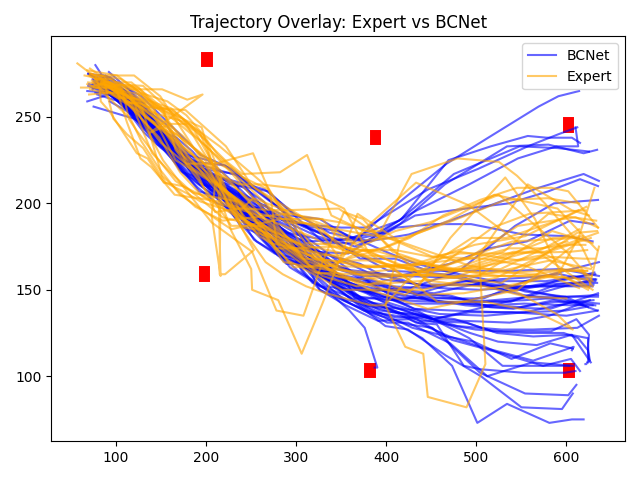
\includegraphics[width=0.6\textwidth]{Images/Evaluation/trajectory_overlay.png}
  \caption{Overlaying plot of the trajectories.}
  \label{fig:trajectory_overlay}
\end{figure}

\subsection{Mean Velocity Comparison}

Comparison between velocity profiles of the expert and the trained model is represented in \autoref{fig:velocity_profiles}. The average linear velocity of the JetBot throughout the whole trajectory was also analyzed:

\begin{itemize}
  \item \textbf{Mean velocity of BCNet:} $0.14$ m/s
  \item \textbf{Mean velocity of Expert:} $0.17$ m/s
\end{itemize}

This result shows that while the BCNet-driven JetBot was capable of navigating the environment, it tended to move more cautiously (i.e., slower) than the expert. This behavior is typical in behavioral cloning approaches, especially in cases of errors during training or poorly constructed dataset \autocite{bühler2020drivingghostsbehavioralcloning}.

\begin{figure}[H]
  \centering
  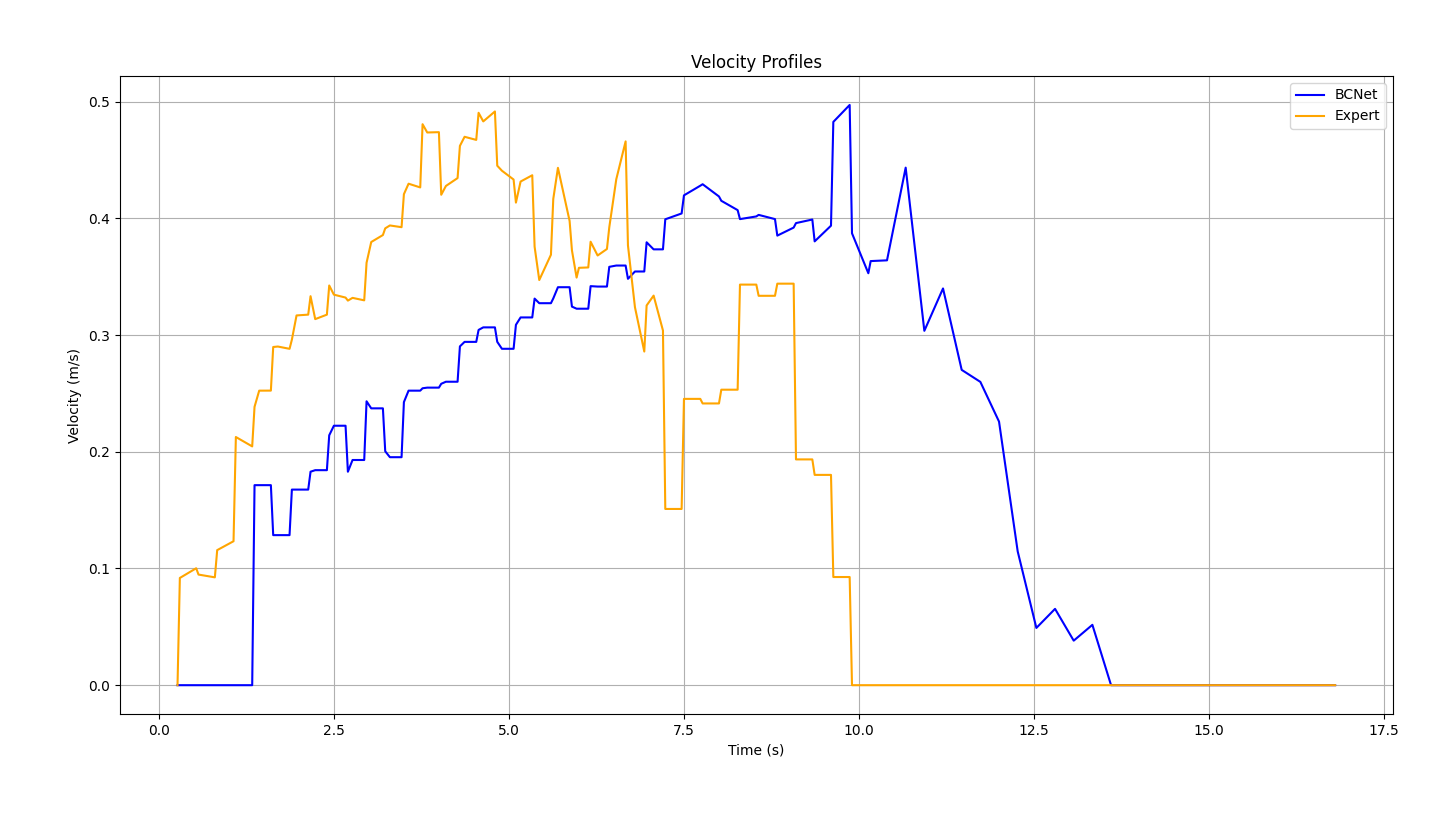
\includegraphics[width=0.8\textwidth]{Images/Evaluation/velocity_profiles.png}
  \caption{Relation between mean velocity and time.}
  \label{fig:velocity_profiles}
\end{figure}

\section{Summary of Evaluation Metrics}

\begin{table}[H]
  \centering
  \caption{Trajectory Evaluation Metrics}
  \label{tab:evaluation_metrics}
  \begin{tabular}{|l|c|}
    \hline
    \textbf{Metric} & \textbf{Value} \\
    \hline
    Davies–Bouldin Index & 1.779 \\
    Silhouette Score (X-axis) & 0.49 \\
    Silhouette Score (Y-axis) & 0.32 \\
    Mean Velocity (BCNet) & 0.14 m/s \\
    Mean Velocity (Expert) & 0.17 m/s \\
    \hline
  \end{tabular}
\end{table}

\chapter{Conclusion and Future Work}
\label{cha:Conclusion}

\section{Conclusion}

Addressing the main research questions:

\begin{enumerate}
  \item \textbf{Can the model be trained using Behavioral Cloning to demonstrate human performance or even surpass it in the first difficulty?} \\
    The evaluation results demonstrate that the behavioral cloning model successfully replicated the expert’s navigational behavior to a considerable degree. The relatively low Davies–Bouldin index and moderate silhouette scores indicate that BCNet produced trajectories with structural patterns comparable to those of the expert.

    However, while BCNet with LSTM layers performs decently in the early stages of the course due to its conservative control, it struggles in later phases, where minor prediction errors compound. This suggests that more diverse training data or alternative methods, such as DAgger, may be necessary to enhance robustness in varied environments.

  \item \textbf{Can the model be sufficiently generalized using behavioral cloning to demonstrate human performance or even surpass it in the second difficulty?} \\
    Unfortunately, the success rate of the BCNet-driven JetBot was 0\% under the conditions of the second difficulty level. This clearly indicates that the model failed to generalize to spatial variations it had not encountered during training. This limitation is a well-known challenge in behavioral cloning (BC) \autoref{NIPS1988_812b4ba2}. Since BC relies heavily on supervised learning from expert trajectories, it tends to perform poorly when encountering states that lie outside of the training distribution. The lack of corrective feedback during training means the model is ill-equipped to recover from novel or slightly off-distribution states, especially in tasks involving obstacle avoidance from unfamiliar angles or trajectories.

  \item \textbf{Can the Inverse Reinforcement Learning (IRL) approach eliminate the expected weaknesses of the Behavioral Cloning approach in mastering the course on both difficulty levels and contribute to successfully mastering the course?} \\
    As this thesis did not provide an opportunity to explore this question empirically, potential solutions will be discussed in \autoref{sec:future_work}.
\end{enumerate}

\section{Future Work}
\label{sec:future_work}

Based on the findings and limitations of this study, several clear directions for future research can be identified to improve the performance and generalization:

\begin{enumerate}
  \item \textbf{Increase the Size and Variety of Training Data} \\
    To improve the model’s ability to generalize, a larger dataset should be collected. Especially the dataset for the second difficulty should include a wider range of initial conditions, obstacle arrangements, and environmental variations. Previous research \autocite{KALRA2016182} shows that the amount of high-quality data needed for autonomous vehicle to operate with decent precision should be very high.

  \item \textbf{Use More Robust Training Methods like Dataset Aggregation (DAgger)} \\
    Since behavioral cloning struggles with unfamiliar states and error accumulation, another possible direction is to explore interactive learning methods like DAgger \autocite{ross2011reduction}. This approach allows the model to receive expert corrections on its own mistakes during training, helping it learn to recover from new or unexpected situations. DAgger could specifically address the compounding errors observed in later course sections. For example, in \autocite{pan2019agileautonomousdrivingusing} a MPPI system that operates using an expensive set of sensors is utilized to collect the data and to train a convolutional neural model to operate on a similar precision by relying only on the camera input.

  \item \textbf{Combine Deep Learning with Model Predictive Path Integral (MPPI) Control} \\
    Integrating deep neural networks with MPPI control methods offers another way to improve navigation. Recent works \autocite{lee2021approximateinversereinforcementlearning, drews2017aggressivedeepdrivingmodel} show that convolutional neural networks can predict cost maps used by MPPI controllers to plan better trajectories. This combination leverages learned perception and model-based planning to handle complex and dynamic environments more effectively.

  \item \textbf{Apply Inverse Reinforcement Learning (IRL) to Learn Reward Functions} \\
    Future research could use inverse reinforcement learning to derive reward functions from expert behavior. Neural networks can be trained to estimate rewards based on state information such as speed, position, and distances to obstacles. These learned rewards can then be used to train policies with on-policy or off-policy reinforcement learning. While on-policy training may require simulation, off-policy methods allow learning from existing data \autocite{arnob2020off}.

\end{enumerate}


% Literaturverzeichnis -----------------------------------------------------
%    Das Literaturverzeichnis wird aus der Datenbank erstellt.
%    Die genaue Verwendung von biblatex wird hier jedoch nicht erklärt.
%    Links:   https://ctan.org/pkg/biblatex?lang=de
%            https://de.overleaf.com/learn/latex/Articles/Getting_started_with_BibLaTeX
% --------------------------------------------------------------------------

\printbibliography

% \setcounter{page}{122}
% \pagenumbering{gobble}
%\pagenumbering{gobble}
\addchap{Declaration of Authorship}
I do solemnly declare that I have written the presented research thesis:

\begin{center}
  \textit{\glqq\titel\grqq}\\[1em]
\end{center}

by myself without undue help from a second person others and without using such tools
other than that specified. Where I have used thoughts from external sources, directly or
indirectly, published or unpublished, this is always clearly attributed. I am aware that
infringement can also subsequently lead to the cancellation of the degree.
\par
\ort, the \eingereicht

\rule[-0.2cm]{5cm}{0.5pt}

\textsc{\autor}
  % Selbständigkeitserklärung

% Anhang -------------------------------------------------------------------
%    Die Contente des Anhangs werden analog zu den Kapiteln inkludiert.
%    Dies geschieht in der Datei Anhang.tex
% --------------------------------------------------------------------------
\appendix
\clearpage
\renewcommand*{\thesection}{\Alph{section}}
\pagenumbering{Roman}
%\include{Content/Anhang}

% Index --------------------------------------------------------------------
%    Zum Erstellen eines Index, die folgende Zeile auskommentieren.
% --------------------------------------------------------------------------
%\printindex    % Index hier einfügen
%\ofoot{}
%\include{Content/Thesen}  % Thesen

\end{document}
